% Este trabalho está licenciado sob a Licença Atribuição-CompartilhaIgual 4.0 Internacional Creative Commons. Para visualizar uma cópia desta licença, visite http://creativecommons.org/licenses/by-sa/4.0/deed.pt_BR ou mande uma carta para Creative Commons, PO Box 1866, Mountain View, CA 94042, USA.

\chapter{Programação Estruturada}\label{cap_progest}
\thispagestyle{fancy}

\hl{No paradigma de programação estruturada, o programa é organizado em blocos de códigos}. Cada bloco tem uma entrada de dados, um processamento (execução de uma tarefa) e produz uma saída.

\begin{figure}[H]
  \centering
  \includegraphics[width=0.4\textwidth]{./cap_progest/dados/fig_fg_bloco/fig}
  \caption{Bloco de processamento.}
  \label{cap_progest:fig:fg_bloco}
\end{figure}

Blocos podem ser colocados em sequência, selecionados com base em condições lógicas, iterados ou colocados dentro de outros blocos (sub-blocos).

\section{Estruturas de um Programa}\label{cap_progest_sec_est}

\hl{Para escrever qualquer programa, apenas três estruturas são necessárias: \emph{sequência}, \emph{seleção/ramificação} e \emph{iteração}}.

\begin{figure}[H]
  \centering
  \includegraphics[width=0.4\textwidth]{./cap_progest/dados/fig_fg_bloco/fig}
  \caption{Bloco de processamento.}
  \label{cap_progest:fig:fg_bloco}
\end{figure}


\subsection{Sequência}

A estrutura de \hl{\emph{sequência}} apenas significa que \hl{os blocos de programação são executados em sequência}. Ou seja, a execução de um bloco começa somente após a finalização do bloco anterior.

\begin{figure}[H]
  \centering
  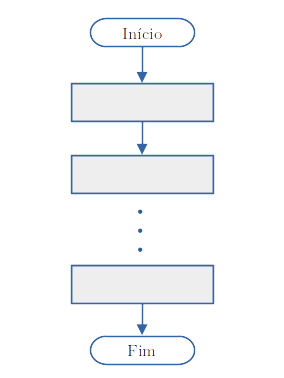
\includegraphics[width=0.4\textwidth]{./cap_progest/dados/fig_fg_sequencia/fig}
  \caption{Estrutura de sequência de blocos.}
  \label{cap_progest:fig:fg_sequencia}
\end{figure}

\begin{ex}
  O seguinte código computada a área do triângulo de base e altura informadas pela(o) usuária(o).
\begin{lstlisting}
#início

# bloco: entrada de dados
base = float(input('Digite a base:\n'))
altura = float(input('Digite a altura\n'))

# bloco: computação da área
area = base*altura/2

# bloco: saída de dados
print(f'Área = {area}')

#fim
\end{lstlisting}

  O código acima está estruturado em três blocos. O primeiro bloco (linhas 3-5) processa a entrada de dados, seu término ocorre somente após a(o) usuária(o) digitar os valores da base e da altura. Na sequência, o bloco (linhas 7-8) faz a computação da área do triângulo e aloca o resultado na variável \lstinline+area+. No que este bloco termina seu processamento, é executado o último bloco (linhas 10-11), que imprime o resultado na tela.
\end{ex}

\subsection{Ramificação}

\hl{Estruturas de ramificação permitem a seleção de um mais blocos com base em condições lógicas}.

\begin{ex}\label{cap_progest_sec_est:ex:ramifica}
  O seguinte código lê um número inteiro digitado pela(o) usuária(o) e imprime uma mensagem no caso do número digitado ser par.
\begin{lstlisting}
#início

# entrada de dados
n = int(input('Digite um número inteiro:\n'))

# ramificação
if (n%2 == 0):
    print(f'{n} é par.')

#término
\end{lstlisting}
  Observamos que, no caso do número digitado não ser par, o programa termina sem nenhuma mensagem ser impressa. Esse é um exemplo de um bloco de ramificação, a instrução de ramificação (linha 7) testa a condição de \lstinline+n+ ser par. Somente no caso de ser verdadeiro, a instrução de impressão (linha 8) é executada. Após e impressão o programa é encerrado. No caso de \lstinline+n+ não ser par, o programa é encerrado sem que a instrução da linha 8 seja executada, i.e. a mensagem não é impressa.

\begin{figure}[H]
  \centering
  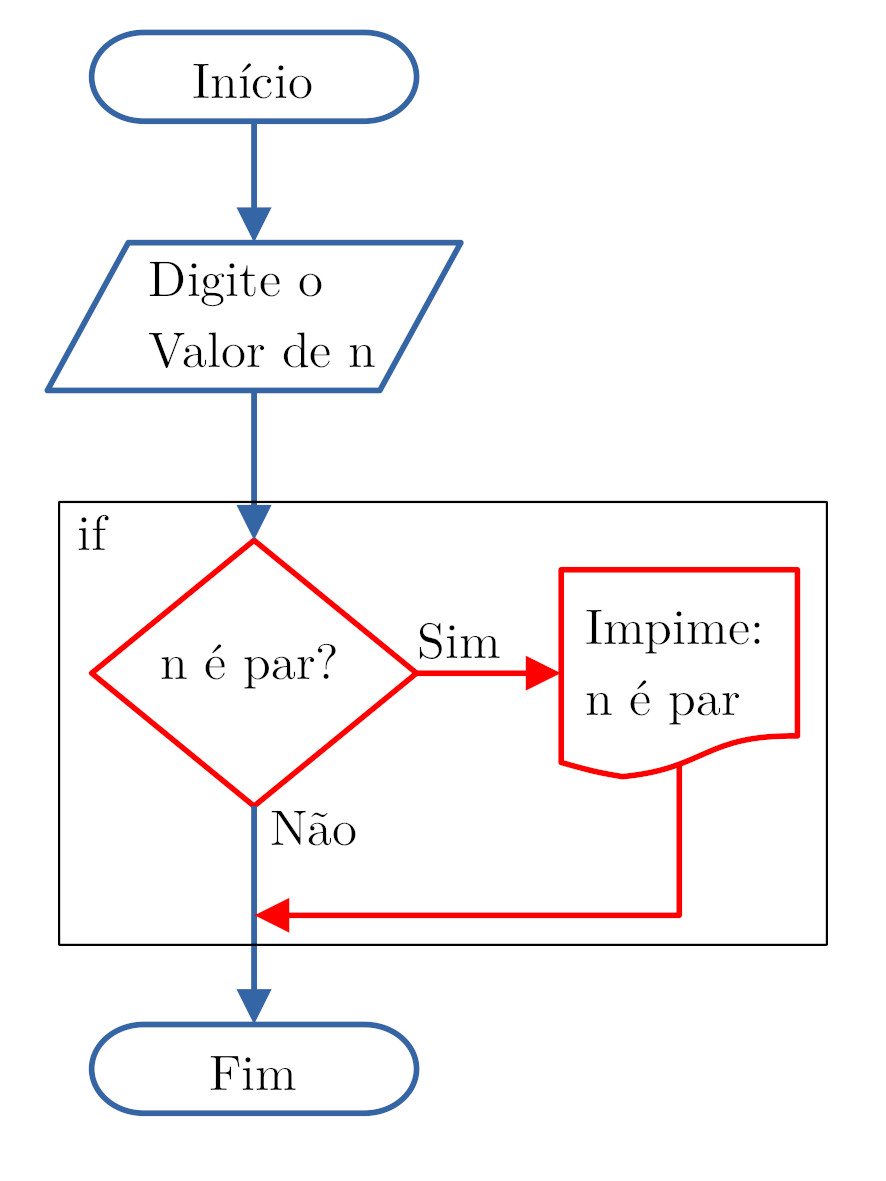
\includegraphics[width=0.5\textwidth]{./cap_progest/dados/fig_fg_ramifica/fig}
  \caption{Fluxograma de uma estrutura de ramificação.}
  \label{cap_progest:fig:fg_ramifica}
\end{figure}
  
\end{ex}

\begin{obs}\normalfont{\hl{(Escopo e indentação.)}}
  Na linguagem {\python}, a \href{https://pt.wikipedia.org/wiki/Indenta\%C3\%A7\%C3\%A3o}{indentação} indica o \emph{escopo}, i.e. o início e fim do bloco de instruções que pertencem a ramificação. No Exemplo \ref{cap_progest_sec_est:ex:ramifica}, o escopo da instrução \lstinline+if+ é apenas a linha 8.
\end{obs}

\subsection{Repetição}

\hl{Instruções de repetição permitem que um mesmo bloco seja processado várias vezes em sequência}. Em {\python}, há duas instruções de repetição disponíveis: \lstinline+for+ e \lstinline+while+. 

\subsubsection{\lstinline+for+}

A instrução \hl{{\lstinline+for+} permite que um bloco seja iterado para cada elemento de uma dada coleção de dados}.

\begin{ex}\label{cap_progest_sec_est:ex:for}
  O seguinte código testa a paridade de cada um dos elementos do conjunto $\{-3, -2, -1, 0, 1, 2, 3\}$.
\begin{lstlisting}
#início

# repetição for
for n in {-3, -2, -1, 0, 1, 2, 3}:
    res = (n%2 == 0)
    print(f'{n} é par? ', res)
    
#término
\end{lstlisting}
  A instrução de repetição \lstinline+for+ (linha 4), aloca em \lstinline+n+ um dos elementos do conjunto. Então, executa em sequência o bloco de comandos das linhas 5 e 6. De forma iterada, \lstinline+n+ recebe um novo elemento do conjunto e o bloco das linhas 5 e 6 é novamente executado. A repetição termina quando todos os elementos do conjunto já tiverem sido iterados. O código segue, então, para a linha 7. Não havendo mais instruções, o programa é encerrado.

\begin{figure}[H]
  \centering
  \includegraphics[width=0.6\textwidth]{./cap_progest/dados/fig_fg_for/fig}
  \caption{Fluxograma de uma estrutura de repetição do tipo \lstinline+for+.}
  \label{cap_progest_sec_est:fig:fg_for}
\end{figure}

Assim como no caso de uma instrução de ramificação, \hl{o escopo do {\lstinline+for+} é definido pela indentação do código}. Neste exemplo, o escopo são as linhas 5 e 6.
\end{ex}

\subsubsection{\lstinline+while+}

A instrução \hl{{\lstinline+while+}, permite a repetição de um bloco enquanto uma dada condição lógica é satisfeita}.

\begin{ex}\label{cap_progest_sec_est:ex:while}
  O seguinte código testa a paridade dos números inteiros compreendidos de $-3$ a $3$.
\begin{lstlisting}
#início

n = -3

# repetição: while
while (n <= 3):
    res = (n%2 == 0)
    print(f'{n} é par?', res)
    n += 1
    
#término
\end{lstlisting}
  A instrução de repetição \lstinline+while+ faz com que o bloco de processamento definido pelas linhas 7-9 seja executado de forma sequencial enquanto o valor de \lstinline+n+ for menor ou igual a 3. No caso dessa condição ser verdadeira, o bloco (linhas 7-9) é executado e, então a condição é novamente verificada. No caso da condição ser falsa, esse bloco não é executado e o código segue para a linha 10. Não havendo mais nenhuma instrução, o programa é encerrado.

  \begin{figure}[H]
    \centering
    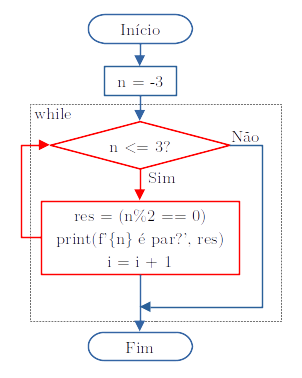
\includegraphics[width=0.6\textwidth]{./cap_progest/dados/fig_fg_while/fig}
    \caption{Fluxograma de uma estrutura de repetição do tipo \lstinline+while+.}
    \label{cap_progest_sec_est:fig:fg_while}
  \end{figure}

  Observamos que, neste exemplo, \hl{o escopo da instrução {\lstinline+while+}} são as linhas 7-9, \hl{determinado indentação do código}.
\end{ex}

\subsection{Exercícios}

\begin{exer}
  Seja a reta de equação
  \begin{equation}
    y = ax + b.
  \end{equation}
  Assumindo $a=2$ e $b=-3$, o seguinte código foi desenvolvido para computar o ponto $x$ de interseção da desta reta com o eixo das abscissas.
\begin{lstlisting}
x = -b/(2*a)
a = 2
b = -3
print(x)
\end{lstlisting}
  Identifique e explique os erros desse código. Então, apresente uma versão corrigida.
\end{exer}
\begin{resp}
\begin{lstlisting}
a = 2
b = -3
x = -b/(2*a)
print(x)
\end{lstlisting}
\end{resp}

\begin{exer}\label{cap_progest_sec_est:exer:ramifica_reta}
  Seja a reta de equação
  \begin{equation}
    y = ax + b.
  \end{equation}
  Faça um fluxograma de um programa em que a(o) usuária(o) entra com os valores de $a$ e $b$. No caso de $a\neq 0$, o programa computa e imprime o ponto $x$ da interseção dessa reta com o eixo das abscissas.
\end{exer}
\begin{resp}
  Dica: consulte o Exemplo \ref{cap_progest_sec_est:ex:ramifica}.
\end{resp}

\begin{exer}
  Implemente o código referente ao fluxograma criado no Exercício \ref{cap_progest_sec_est:exer:ramifica_reta}.
\end{exer}
\begin{resp}
\begin{lstlisting}
a = float(input('Digite o valor de a:\n'))
b = float(input('Digite o valor de b:\n'))
if (a != 0):
    x = -b/(2*a)
    print(f'Ponto de interseção com o eixo x = {x}')
\end{lstlisting}
\end{resp}

\begin{exer}\label{cap_progest_sec_est:exer:for}
  Faça o fluxograma de um programa que usa de um bloco de repetição \lstinline+for+ para percorrer o conjunto
  \begin{equation}
    A = \{-4, -3, -2, -1, 0, 1, 2, 3, 4\}.
  \end{equation}
  A cada iteração, o programa imprime \lstinline+True+ ou \lstinline+False+ conforme o elemento seja ímpar ou não.
\end{exer}
\begin{resp}
  Dica: consulte o Exemplo \ref{cap_progest_sec_est:ex:for}.
\end{resp}

\begin{exer}
  Implemente o código referente ao fluxograma criado no Exercício \ref{cap_progest_sec_est:exer:for}.
\end{exer}
\begin{resp}
\begin{lstlisting}
A = {-4, -3, -2, -1, \
     0, 1, 2, 3, 4}
for x in A:
    res = (x % 2 != 0)
    print(f'{x} é ímpar? {res}')
\end{lstlisting}
\end{resp}

\begin{exer}\label{cap_progest_sec_est:exer:while}
  Faça um fluxograma análogo ao do Exercício \ref{cap_progest_sec_est:exer:for} que use a instrução de repetição \lstinline+while+ no lugar de \lstinline+for+.
\end{exer}
\begin{resp}
  Dica: consulte o Exemplo \ref{cap_progest_sec_est:ex:while}.
\end{resp}

\begin{exer}
  Implemente um código referente ao fluxograma criado no Exercício \ref{cap_progest_sec_est:exer:while}.
\end{exer}
\begin{resp}
\begin{lstlisting}
A = {-4, -3, -2, -1, \
     0, 1, 2, 3, 4}
n = -4
while (n <= 4):
    res = (n % 2 != 0)
    print(f'{n} é ímpar? {res}')
    n += 1
\end{lstlisting}
\end{resp}

\section{Instruções de Ramificação}\label{cap_progest_sec_ramifica}

\hl{Instruções de ramificação permitem a seleção de blocos de processamento com base em condições lógicas}.

\subsection{Instrução \lstinline+if+}

\hl{A instrução de ramificação {\lstinline+if+} permite a seleção de um bloco de processamento com base em uma condição lógica}.

\begin{figure}[H]
  \centering
  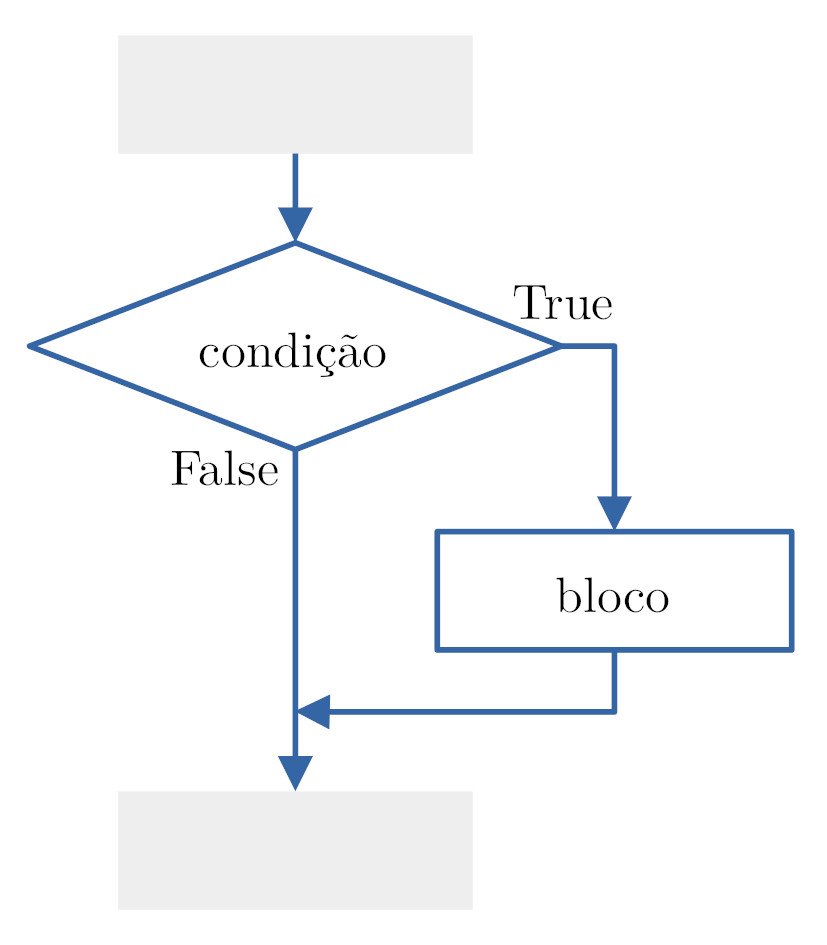
\includegraphics[width=0.5\textwidth]{./cap_progest/dados/fig_fg_if/fig}
  \caption{Fluxograma de uma ramificação \lstinline+if+.}
  \label{cap_progest_sec_ramifica:fig:fg_if}
\end{figure}

Em {\python}, a \hl{instrução {\lstinline+if+}} tem a seguinte \hl{sintaxe}:
\begin{lstlisting}
bloco_anterior
if (condição):
    bloco_0
bloco_posterior
\end{lstlisting}
Se a {\lstinline+condição+} é verdadeira ({\lstinline+True+}), o bloco (linha 3) é executado. Caso contrário, este bloco não é executado e o fluxo de processamento salta da linha 2 para a linha 6. O \hl{\emph{escopo} do bloco {\lstinline+if+} é determinado pela indentação do código}.

\begin{ex}\label{cap_progest_sec_ramifica:ex:bhaskara_if}
  Seja o polinômio de segundo grau
  \begin{equation}
    p(x) = ax^2 + bx + c.
  \end{equation}
  No caso de existirem, o seguinte código computa as raízes distintas de $p(x)$ para os coeficientes informados pela(o) usuária(o).
\begin{lstlisting}
# entrada de dados
a = float(input('Digite o valor de a:\n'))
b = float(input('Digite o valor de b:\n'))
c = float(input('Digite o valor de c:\n'))

# discriminante
delta = b**2 - 4*a*c

# raízes
if (delta > 0):
    # raízes distintas
    x1 = (-b - delta**0.5)/(2*a)
    x2 = (-b + delta**0.5)/(2*a)
    print(f'x_1 = {x1}')
    print(f'x_2 = {x2}')
\end{lstlisting}
\end{ex}

\subsubsection{Escopo de variáveis}

O \emph{escopo} de uma variável é a região em que ela permanece alocada. \hl{O escopo de variáveis alocadas fora do bloco {\lstinline+if+} inclui este bloco, mas variáveis alocadas no bloco {\lstinline+if+} não permanecem alocadas fora deste}.

\begin{ex}
  No Exemplo \ref{cap_progest_sec_ramifica:ex:bhaskara_if}, o escopo da variável \lstinline+delta+ inicia-se na linha 7 e permanece válido ao longo do resto do programa. Já, o escopo da variável \lstinline+x1+ compreende somente as linhas 12-15 e, análogo para a variável \lstinline+x2+. 
\end{ex}

\subsection{Instrução \lstinline+if-else+}

A instrução \hl{{\lstinline+if-else+} permite a escolha de um bloco ou outro, exclusivamente, com base em uma condição lógica}.

\begin{figure}[H]
  \centering
  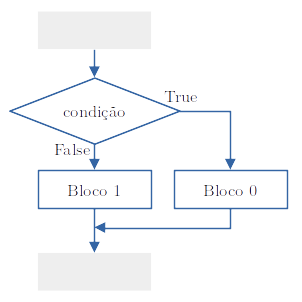
\includegraphics[width=0.7\textwidth]{./cap_progest/dados/fig_fg_else/fig}
  \caption{Fluxograma de uma ramificação \lstinline+if-else+.}
  \label{cap_progest_sec_ramifica:fig:fg_else}
\end{figure}

Em {\python}, a instrução \lstinline+if-else+ tem a seguinte sintaxe:
\begin{lstlisting}
bloco_anterior
if (condição):
    bloco_0
else:
    bloco_1
bloco_posterior
\end{lstlisting}

Se a {\lstinline+condição+} for verdadeira ({\lstinline+True+}) o {\lstinline+bloco 0+} é executado, senão o {\lstinline+bloco 1+} é executado.

\begin{ex}
  Seja o polinômio de segundo grau
  \begin{equation}
    p(x) = ax^2 + bx + c.
  \end{equation}
  Se existirem, o seguinte código computa as raízes reais do polinômio, senão imprime mensagem informado que elas não são reais.
\begin{lstlisting}
# entrada de dados
a = float(input('Digite o valor de a:\n'))
b = float(input('Digite o valor de b:\n'))
c = float(input('Digite o valor de c:\n'))

# discriminante
delta = b**2 - 4*a*c

# raízes
if (delta >= 0):
    x1 = (-b - delta**0.5)/(2*a)
    x2 = (-b + delta**0.5)/(2*a)
    print(f'x_1 = {x1}')
    print(f'x_2 = {x2}')
else:
    print('Não tem raízes reais.')
\end{lstlisting}
\end{ex}

\subsubsection{Instrução \lstinline+if-else+ em linha}

Por praticidade, {\python} também tem a sintaxe \lstinline+if-else+ em linha:
\begin{lstlisting}
x = valor if True else outro_valor
\end{lstlisting}

\begin{ex}
  O valor absoluto de um número real $x$ é
  \begin{equation}
    |x| := \left\{
      \begin{array}{ll}
        x &, x\geq 0,\\
        -x &, x<0
      \end{array}
    \right.
  \end{equation}
  O seguinte código, computa o valor absoluto\footnote{{\python} tem a função \href{https://docs.python.org/3/library/functions.html\#abs}{\lstinline+abs()+} que computa o valor absoluto de um número.} de um número dado pela(o) usuária(o).
\begin{lstlisting}
x = float(input('Digite o valor de x:\n'))
abs_x = x if (x>=0) else -x
print(f'|x| = {abs_x}')
\end{lstlisting}
\end{ex}

\subsection{Instrução \lstinline+if-elif+}

\hl{A instrução {\lstinline+if-elif+} permite a seleção condicional de blocos, sem impor a necessidade da execução de um deles}.

\begin{figure}[H]
  \centering
  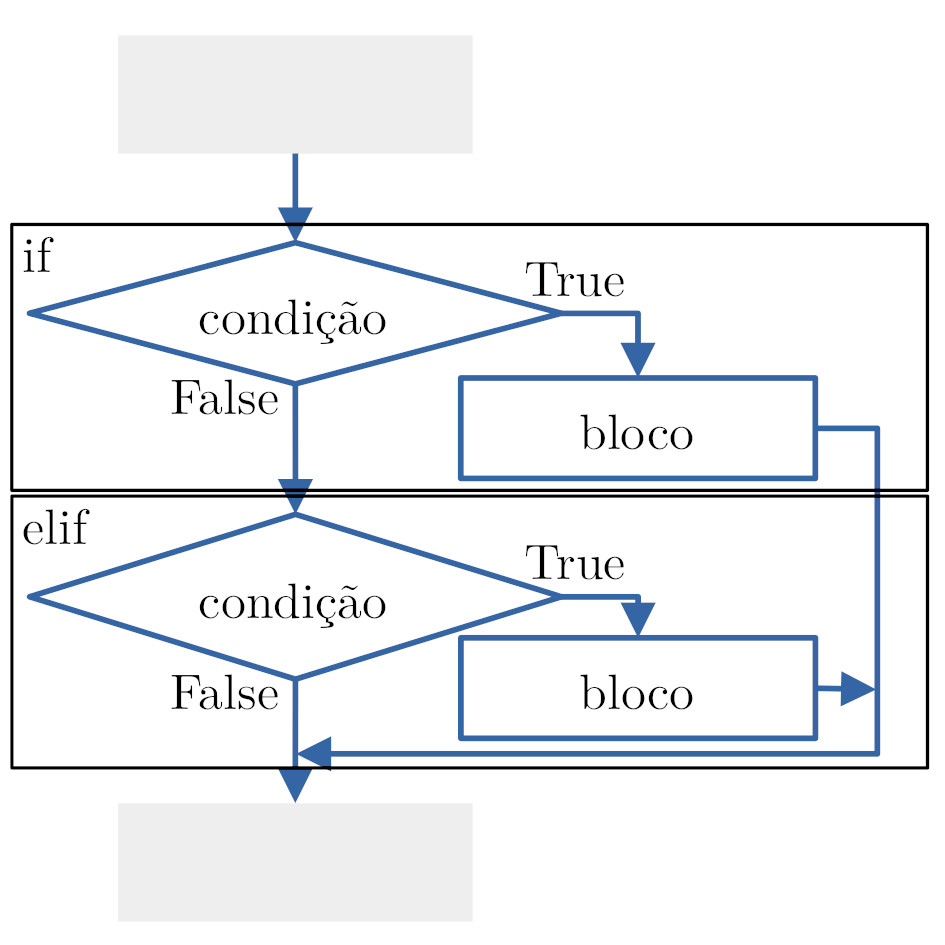
\includegraphics[width=0.7\textwidth]{./cap_progest/dados/fig_fg_elif/fig}
  \caption{Fluxograma de uma ramificação \lstinline+if-elif+.}
  \label{cap_progest_sec_ramifica:fig:fg_elif}
\end{figure}

Em {\python}, a instrução \lstinline+if-elif+ tem a seguinte sintaxe:
\begin{lstlisting}
bloco_anterior
if (condição_0):
    bloco_0
elif (condição 1):
    bloco_1
bloco posterior
\end{lstlisting}
Se a \lstinline+condição_0+ for verdadeira (lstinline+True+), o \lstinline+bloco_0+ é executado. Senão, se a \lstinline+condição_1+ for verdadeira (\lstinline+True+) o \lstinline+bloco_1+ é executado. No caso de ambas as condições serem falsas (\lstinline+False+), os blocos \lstinline+bloco_0+ e \lstinline+bloco_1+ não são executados e o fluxo de processamento segue a partir da linha 6.

\begin{ex}
  Seja o polinômio de segundo grau
  \begin{equation}
    p(x) = ax^2 + bx + c.
  \end{equation}
  Conforme o caso, o seguinte código computa a raiz dupla do polinômio ou suas raízes distintas, a partir dos coeficientes informados pela(o) usuária(o).
\begin{lstlisting}
# entrada de dados
a = float(input('Digite o valor de a:\n'))
b = float(input('Digite o valor de b:\n'))
c = float(input('Digite o valor de c:\n'))

# discriminante
delta = b**2 - 4*a*c

# raízes
if (delta > 0):
    x1 = (-b - delta**0.5)/(2*a)
    x2 = (-b + delta**0.5)/(2*a)
    print('Raízes reais distintas:')
    print(f'x_1 = {x1}')
    print(f'x_2 = {x2}')
elif (delta == 0):
    print('Raiz dupla:')
    x = -b/(2*a)
    print('x_1 = x_2 = {x}')
\end{lstlisting}
\end{ex}

\subsection{Instrução \lstinline+if-elif-else+}

A instrução \lstinline+if-elif-else+ permite a seleção condicional de blocos, sendo que ao menos um bloco será executado. Em {\python}, sua sintaxe é:
\begin{lstlisting}
bloco_anterior
if (condição_0):
    bloco_0
elif (condição_1):
    bloco_1
else:
    bloco_2
bloco posterior
\end{lstlisting}
Se a \lstinline+condição_0+ for verdadeira (\lstinline+True+), então o \lstinline+bloco_0+ é executado. Senão, se a \lstinline+condição_1+ for verdadeira (\lstinline+True+), então o \lstinline+bloco_1+ é executado. Senão, o \lstinline+bloco_2+ é executado.

\begin{ex}
  Seja o polinômio de segundo grau
  \begin{equation}
    p(x) = ax^2 + bx + c.
  \end{equation}
  Conforme o caso (raízes distintas, raiz dupla ou raízes complexas), o seguinte código computa as raízes  desse polinômio, a partir dos coeficientes informados pela(o) usuária(o).
\begin{lstlisting}
# entrada de dados
a = float(input('Digite o valor de a:\n'))
b = float(input('Digite o valor de b:\n'))
c = float(input('Digite o valor de c:\n'))

# discriminante
delta = b**2 - 4*a*c

# raízes
if (delta > 0):
    # raízes distintas
    x1 = (-b - delta**0.5)/(2*a)
    x2 = (-b + delta**0.5)/(2*a)
    print('Raízes reais distintas:')
    print(f'x_1 = {x1}')
    print(f'x_2 = {x2}')
elif (delta == 0):
    # raiz dupla
    x = -b/(2*a)
    print('Raiz dupla:')
    print('x_1 = x_2 = {x}')
else:
    # raízes complexas
    # parte real
    rea = -b/(2*a)
    # parte imaginária
    img = (-delta)**0.5/(2*a)
    x1 = rea - img*1j
    x2 = rea + img*1j
    print('Raízes complexas:')
    print(f'x_1 = {x1}')
    print(f'x_2 = {x2}')
\end{lstlisting}
\end{ex}

\subsection{Múltiplos Casos}

\hl{Pode-se encadear instruções {\lstinline+if-elif-elif-...-elif[-else]+} para a seleção condicional entre múltiplos blocos}.

\begin{ex}
  Sejam as circunferências de equações:
  \begin{align}
    c_1&: (x-a_1)^2 + (y-b_1)^2 = r_1,\\
    c_2&: (x-a_1)^2 + (y-b_1)^2 = r_2.
  \end{align}
  Conforme entradas dadas por usuária(o), o seguinte código informa se um dado ponto $(x, y)$ pertence: à interseção dos discos determinados por $c_1$ e $c_2$, apenas ao disco determinado por $c_1$, apenas ao disco determinado por $c_2$ ou a nenhum desses discos.
\begin{lstlisting}
# entrada de dados
print('c1: (x-a1)**2 + (y-b1)**2 = r1')
a1 = float(input('Digite o valor de a1:\n'))
b1 = float(input('Digite o valor de b1:\n'))
r1 = float(input('Digite o valor de r1:\n'))
print('c2: (x-a2)**2 + (y-b2)**2 = r1')
a2 = float(input('Digite o valor de a2:\n'))
b2 = float(input('Digite o valor de b2:\n'))
r2 = float(input('Digite o valor de r2:\n'))
print('Ponto de interesse (x,y).')
x = float(input('Digite o valor de x:\n'))
y = float(input('Digite o valor de y:\n'))

# pertence ao disco c1?
c1 = (x-a1)**2 + (y-b1)**2 <= r1
# pertence ao disco c2?
c2 = (x-a2)**2 + (y-b2)**2 <= r2

# imprime resultado
if (c1 and c2):
    print(f'({x}, {y}) pertence à interseção dos discos.')
elif (c1):
    print(f'({x},{y}) pertence ao disco c1.')
elif (c2):
    print(f'({x},{y}) pertence ao disco c2.')
else:
    print(f'({x},{y}) não pertence aos discos.')
\end{lstlisting}
\end{ex}


\subsection{Exercícios}

\begin{exer}
  Seja a equação de reta
  \begin{equation}
    ax + b = 0.
  \end{equation}
  Dados coeficientes $a \neq 0$ e $b$ informados por usuária(o), crie um código que imprime o ponto de interseção dessa reta com o eixo das abscissas. O código não deve tentar computar o ponto no caso de $a=0$. 
\end{exer}
\begin{resp}
\begin{lstlisting}
# entrada de dados
a = float(input('Digite o valor de a:\n'))
b = float(input('Digite o valor de b:\n'))

# computação
if (a != 0):
    x = -b/a
    y = a*x + b
    print(f'Intercepta eixo-x em: ({x}, {y}).')
\end{lstlisting}
\end{resp}

\begin{exer}
  Considere o seguinte código.
\begin{lstlisting}
n = int(intput('Digite um número inteiro:\n')
if (n % 2 == 0):
    m = 1
n = n + m
print(n)
\end{lstlisting}
  A ideia é que, se $n$ for ímpar, o código imprime $n$, caso contrário, imprime $n+1$. Este código contém erro. Identifique e explique-o, então proponha uma versão funcional.
\end{exer}
\begin{resp}
\begin{lstlisting}
n = int(intput('Digite um número inteiro:\n')
m = 0
if (n % 2 == 0):
    m = 1
n = n + m
print(n)
\end{lstlisting}
\end{resp}

\begin{exer}
  Considere a equação da circunferência
  \begin{equation}
    c: (x-a)^2 + (y-b)^2 = r.
  \end{equation}
  Com dados informados por usuária(o), desenvolva um código que informe se um dado ponto $(x, y)$ pertence ou não ao disco determinado por $c$.
\end{exer}
\begin{resp}
\begin{lstlisting}
# entrada de dados
print('Circunferência c:')
a = float(input('Digite o valor de a:\n'))
b = float(input('Digite o valor de b:\n'))
r = float(input('Digite o valor de r:\n'))
print('Ponto (x, y):')
x = float(input('Digite o valor de x:\n'))
y = float(input('Digite o valor de y:\n'))

# resultado
if ((x-a)**2 + (y-b)**2 <= r):
    print(f'({x}, {y}) pertence ao disco.')
else:
    print(f'({x}, {y}) não pertence ao disco.')
\end{lstlisting}
\end{resp}

\begin{exer}\label{cap_progest_sec_ramifica:exer:intercep_retas}
  Sejam informadas por usuária(o) os coeficientes das retas
  \begin{align}
    r_1&: a_1x + b_1 = 0,\\
    r_2&: a_2x + b_2 = 0.
  \end{align}
  Crie um código que informe se as retas são paralelas. Caso contrário, o código imprime o ponto de interseção delas.
\end{exer}
\begin{resp}
\begin{lstlisting}
# entrada de dados
print('r1: a1*x + b1 = 0')
a1 = float(input('Digite o valor de a1:\n'))
b1 = float(input('Digite o valor de b1:\n'))
print('r2: a2*x + b2 = 0')
a2 = float(input('Digite o valor de a2:\n'))
b2 = float(input('Digite o valor de b2:\n'))

# resultado
if (a1 == a2):
    print('r1 // r2')
else:
    x = (b1-b2)/(a2-a1)
    y = a1*x + b1
    print('Ponto de interseção: ({x}, {y}).')
\end{lstlisting}
\end{resp}

\begin{exer}
  Refaça o código do Exercício \ref{cap_progest_sec_ramifica:exer:intercep_retas} de forma a incluir o caso em que as retas sejam coincidentes. Ou seja, o código deve informar os seguintes casos: retas paralelas não coincidentes, retas coincidentes ou, caso contrário, ponto de interseção das retas.
\end{exer}
\begin{resp}
\begin{lstlisting}
# entrada de dados
print('r1: a1*x + b1 = 0')
a1 = float(input('Digite o valor de a1:\n'))
b1 = float(input('Digite o valor de b1:\n'))
print('r2: a2*x + b2 = 0')
a2 = float(input('Digite o valor de a2:\n'))
b2 = float(input('Digite o valor de b2:\n'))

# resultado
if (a1 == a2):
    if (b1 == b2):
        print('r1 = r2')
    else:
        print('r1 // r2 e r1 != r2')
else:
    x = (b1-b2)/(a2-a1)
    y = a1*x + b1
    print('Ponto de interseção: ({x}, {y}).')
\end{lstlisting}
\end{resp}

\begin{exer}
  Sejam a parábola de equação
  \begin{equation}
    a_1x^2 + a_2x + a_3 = 0
  \end{equation}
  e a reta
  \begin{equation}
    b_1x + b_2 = 0.
  \end{equation}
  Conforme os coeficientes dados por usuária(o), desenvolva um código que imprime o(s) ponto(s) de interseção da reta com a parábola. O código deve avisar os casos em que: há apenas um ponto, há dois pontos ou não há ponto de interseção.
\end{exer}
\begin{resp}
\begin{lstlisting}
# entrada de dados
print('Coeficientes da parábola')
print('a1*x**2 + a2*x + a3 = 0')
a1 = float(input('Digite o valor de a1:\n'))
a2 = float(input('Digite o valor de a2:\n'))
a2 = float(input('Digite o valor de a3:\n'))

print('Coeficientes da reta')
print('b1*x + b2 = 0')
b1 = float(input('Digite o valor de b1:\n'))
b2 = float(input('Digite o valor de b2:\n'))

# discriminante da equação
# a1*x**2 + (a2-b1)*x + (a3-b2) = 0
delta = (a2-b1)**2 - 4*a1*(a3-b2)

# ponto(s) de interseção
if (delta == 0):
    x = (b1-a2)/(2*a1)
    y = b1*x + b2
    print('Ponto de interseção:')
    print(f'({x}, {y})')
elif (delta > 0):
    x1 = ((b1-a2) - delta**2)/(2*a1)
    y1 = b1*x1 + b2
    x2 = ((b1-a2) + delta**2)/(2*a1)
    y2 = b1*x2 + b2
    print('Pontos de interseção:')
    print(f'({x1}, {y1}), ({x2}, {y2})')
else:
    print('Não há ponto de interseção.')
\end{lstlisting}
\end{resp}

\begin{exer}
  Com dados informados por usuária(o), sejam as circunferências de equações
  \begin{align}
    c_1&: (x-a_1)^2 + (y-b_1)^2 = r_1,\\
    c_2&: (x-a_2)^2 + (y-b_2)^2 = r_2.
  \end{align}
  Desenvolva um código que informe a(o) usuária(o) dos seguintes casos: $c_1$ e $c_2$ são coincidentes, $c_1\cap c_2$ tem dois pontos, $c_1\cap c_2$ tem somente um ponto, $c_1\cap c_2 = \emptyset$.
\end{exer}
\begin{lstlisting}
# entrada de dados
print('c1: (x-a1)**2 + (y-b1)**2 = r1')
a1 = float(input('Digite o valor de a1:\n'))
b1 = float(input('Digite o valor de b1:\n'))
r1 = float(input('Digite o valor de r1:\n'))
print('c2: (x-a2)**2 + (y-b2)**2 = r1')
a2 = float(input('Digite o valor de a2:\n'))
b2 = float(input('Digite o valor de b2:\n'))
r2 = float(input('Digite o valor de r2:\n'))

# verificações
if (((a1==a2) and (b1==b2)) and (r11==r2)):
    print('c1 = c2')
else:
    # distância entre os centros
    dist = ((a2-a1)**2 + (b2-b1)**2)**0.5
    if (abs(dist - (r1+r2)) < 1e-15):
        print('c1 & c2 têm um único ponto de interseção.')
    elif (dist < r1+r2):
        print('c1 & c2 têm dois pontos de interseção.')
    else:
        print('c1 & c2 não tem ponto de interseção.')
\end{lstlisting}

\begin{exer}
  Crie uma calculadora simples. A(o) usuária(o) entra com dois números decimais \lstinline+x+ e \lstinline+y+ e uma das seguintes operações: \lstinline!+!, \lstinline+-+, \lstinline+*+ ou \lstinline+/+. Então, o código imprime o resultado da operação.
\end{exer}
\begin{resp}
\begin{lstlisting}
# entrada de dados
x = float(input('Digite o valor de x:\n'))
op = input('Digite uma das operações +, -, * ou /:\n')
y = float(input('Digite o valor de y:\n'))

# calcula
if (op == '+'):
    print(f'{x} ' + op + f' {y} = {x+y}')
elif (op == '-'):
    print(f'{x} ' + op + f' {y} = {x-y}')
elif (op == '*'):
    print(f'{x} ' + op + f' {y} = {x*y}')
elif (op == '/'):
    print(f'{x} ' + op + f' {y} = {x/y}')
else:
    print('Desculpa, não entendi!')
\end{lstlisting}
\end{resp}

\section{Instruções de Repetição}\label{cap_progest_sec_repete}

[[tag:construcao]]

\subsection{Instrução \lstinline+while+}

[[tag:construcao]]

\subsection{Instrução \lstinline+for+}

[[tag:construcao]]

\subsection{Exercícios}

[[tag:construcao]]